\documentclass[sigconf]{acmart}

\usepackage{booktabs} % For formal tables

%% -- Local style additions
% \usepackage{times}
\usepackage{xcolor}
\usepackage{siunitx}
\usepackage{multirow}
\usepackage{xspace}
\usepackage{balance}
\usepackage[font=rm]{caption}
\usepackage{algorithm}
\usepackage[noend]{algpseudocode}
\usepackage{verbatim}
\usepackage{graphicx}
\usepackage{tabularx}
\usepackage{enumitem}
\usepackage{shortvrb}
\usepackage{tikz}
\usetikzlibrary{matrix,decorations.pathreplacing,calc,positioning}
\renewcommand{\topfraction}{0.9}
\renewcommand{\bottomfraction}{0.9}
\renewcommand{\textfraction}{0.1}
%% configure number representation defaults
\sisetup{
group-separator = {,},
round-mode = places,
round-precision = 2
}%

\newcommand{\method}[1]{{\small\sf{#1}}}
\newcommand{\gb}[1]{{\mbox{$#1$~GiB}}}
\newcommand{\mb}[1]{{\mbox{$#1$~MiB}}}
\newcommand{\kb}[1]{{\mbox{$#1$~kiB}}}

\newcommand{\tab}{\makebox[2em]{~}}
\newcommand{\var}[1]{\mbox{\emph{#1}}}
\newcommand{\vars}[1]{\mbox{\scriptsize\emph{#1}}}
\newcommand{\sym}[1]{\mbox{\small{\sf{#1}}}}
\newcommand{\syms}[1]{\mbox{\scriptsize{\sf{#1}}}}
\newcommand{\bits}[1]{\mbox{\sf{#1}}}
\newcommand{\BigO}[1]{\ensuremath{O\bigl(#1\bigr)}}
\def\D{\hphantom{1}}
\def\C{\hphantom{1,}}

\newcommand{\myparagraph}[1]{\paragraph*{\hspace*{-\parindent}\normalsize\bf#1.}}
\newcommand{\mycaption}[1]{\caption{{\rm{#1}}}}
\newcommand{\myfootnote}[1]{\footnote{{#1}}}

\usepackage{xcolor}
\newcommand{\jane}[1]{{\color{blue}{\bf{Jane says:}} \emph{#1}}}
\newcommand{\alistair}[1]{{\color{purple}{\bf{Alistair says:}} \emph{#1}}}
\newcommand{\jack}[1]{{\color{orange}{\bf{Jack says:}} \emph{#1}}}
\newcommand{\todo}[1]{{\color{blue}{[[#1]]}}}

\newcommand{\whatever}{\method{WhatEver}}

\newcommand{\collection}[1]{\method{#1}}
\newcommand{\govtwo}{\collection{Gov2}}
\newcommand{\clueweb}{\collection{ClueWeb09}}
\newcommand{\commoncrawl}{\collection{CC}}

\newcommand{\aftertabspace}{\vspace*{-2ex}}
\newcommand{\afterfigspace}{\vspace*{-0ex}}
\newcommand{\afterpixspace}{\vspace*{-1ex}}

\newcommand{\bzip}{{\method{BZip2}}}
\newcommand{\efopt}{\mbox{\method{EF-opt}}}
\newcommand{\ef}{{\method{EF}}}
\newcommand{\interp}{{\method{Interp}}}
\newcommand{\qmx}{\method{QMX}}
\newcommand{\uef}{\method{UEF}}
\newcommand{\ans}{{\method{ANS}}}
\newcommand{\vbyte}{{\method{VByte}}}
\newcommand{\simple}{{\method{Simple}}}
\newcommand{\packed}{{\method{Packed}}}
\newcommand{\pfor}{\method{PFOR}}
\newcommand{\opf}{\method{Opt-PFOR}}
\newcommand{\vbyteplus}{\method{\vbyte+ANS}}
\newcommand{\simpleplus}{\method{\simple+ANS}}
\newcommand{\packedplus}{\method{\packed+ANS}}
\newcommand{\packedpp}{\method{\packed+ANS2}}
\newcommand{\opfplus}{\method{\opf+ANS}}
\newcommand{\ansmapping}{\mbox{\emph{ANSmsb}}}
\newcommand{\xz}{{\method{XZ}}}
\newcommand{\zlib}{{\method{ZLib}}}
\newcommand{\zstd}{{\method{ZStd}}}
\newcommand{\raw}{{\method{U32}}}

\newcommand{\ddt}{{\ensuremath{d_{t,i}}}}
\newcommand{\fdt}{{\ensuremath{f_{t,i}}}}
\newcommand{\dfdt}{{\ensuremath{\langle \ddt, \fdt\rangle}}}

%% -- End local style additions

% Copyright
\setcopyright{none}
%\setcopyright{acmcopyright}
%\setcopyright{acmlicensed}
%\setcopyright{rightsretained}
%\setcopyright{usgov}
%\setcopyright{usgovmixed}
%\setcopyright{cagov}
%\setcopyright{cagovmixed}


% DOI
\acmDOI{10.1145/000000.000000}

% ISBN
\acmISBN{123-4567-24-567/08/06}

%Conference
\acmConference[COMP90049-Knowlege Technologies, University of Melbourne]{August 2017}
\acmYear{2017}
\copyrightyear{2017}

\acmPrice{15.00}

\settopmatter{printacmref=false, printfolios=false}

\begin {document}
\title{Identifying Tweets with Adverse Drug Reactions}
%% \titlenote{Produces the permission block, and
%%   copyright information}
%% \subtitle{Extended Abstract}
%% \subtitlenote{The full version of the author's guide is available as
%%   \texttt{acmart.pdf} document}

%% As of 17-06-24 authorship and authorship order not yet discussed.

\author{COMP90049 - Knowledge Technologies - Project 2}
%% \orcid{1234-5678-9012}
\affiliation{%
  \institution{The University of Melbourne}
}
\email{}


\begin{abstract}
In this report, we discuss effectiveness of machine learning  algorithms on the problem of tweets containing adverse drug reactions. Firstly, discuss the feature engineering, text normalisation. Then we transition into the analysis phase of the methods, while trying to understand their theoretical differences. We review several machine learning algorithms such as Naive Bayes, Support Vector Machines and Decision Tree. Further, we perform a critical analysis of another study with a similar problem.
\end{abstract}




\keywords{Classification Techniques; Feature Engineering; Support Vector Machine; Decision Tree; Naive Bayes; Perceptron;  Random Forest}

\maketitle

\begin{abstract}
In this report, we discuss effectiveness of machine learning  algorithms on the problem of tweets containing adverse drug reactions. Firstly, discuss the feature engineering, text normalisation. Then we transition into the analysis phase of the methods, while trying to understand their theoretical differences. We review several machine learning algorithms such as Naive Bayes, Support Vector Machines and Decision Tree. Further, we perform a critical analysis of another study with a similar problem.
\end{abstract}


\section{Introduction}
\label{sec-intro}

Capturing of Adverse Drug Reactions (ADR) is of significance importance for multiple reason. The most important being it going unnoticed and thus leading to medical complications. Secondly, this data may not be available elsewhere and offers a valuable perspective. Natural language processing is certainly a challenging task due to the unstructured and informal nature of text. Additionally the complication nature of drugs and their indications is tough to judge. In this paper our focus is on a.set of tweets provided to us. With substantial pre-processing, feature engineering, vector space creation; we attempt to critically evaluate different machine learning algorithms.









\section{Text Normalisation Techniques}
\label{sec-background}

\subsection{Text Pruning}
This raw text of $train.txt$ and $dev.txt$ provides us with our first problem. We need to transform our raw text data into a set of features that describe qualitative concepts in a quantitative way, we call this as feature vector space. In our case, that will be a 1/-1 coding strategy: Yes or No. For the this project, we process our features such that they do not include words beginning with {\#} and {$@$} and we are more concerned with English words. We use {\citet{gm14}} for text normalisation.



\subsection{Feature Engineering}
Before we begin analysing our tokens, we would want to categorise and extract the tokens which we would want to consider as attributes. Our focus is to combine attributes into various n- gram categories, such as 1 Gram, 2 Gram, 3 Gram; defining them as non-gram attributes. We use $tokens.txt$ and $dev.txt$ for extracting the attributes. We maintain the token in a line-by-line format in $N$$-$$gramtoken.txt$, where ${N=1,2,3}$. This is perform in the $n-gram.py$ where we can pass N as a parameter and the script returns a feature vector space of the entire file that is being parsed. 

Feature subset selection is the process of identifying and removing as many irrelevant and redundant features as possible. This reduces the dimensionality of the data and enables data mining algorithms to operate faster and more effectively.
For this we apply \textbf{LASSO} ({least absolute shrinkage and selection operator}) and we make an interesting observation. 

In our observation {neck, pic, skin, restless and zombie} can produce quite a high number of correctly classified instances. To put things in perspective, using the Support vector machine, we received 82.15\% correctly classified instances when classifying $dev$ keeping $train$ as the prepossessing module, while just using particularly these 5 words gives us a staggering, 89.68 \% correctly classified instances and 10.316 \% incorrectly classified instances. The other parameters such as root mean square error and relative absolute error also take a substantial decrease above 45\%.However, it is quite obvious that these 5 features alone may not be sufficient for us to classify the unknown $test$ classes and we need some number of instances. However, this observation tells us something about the data i.e. there is a clear bias in the weightage each of the 92 attribute has and perhaps identifying the key attributes can help us in forming new set of attributes. 

We further explore the 'Select attributes' tab in the $WEKA$ explorer, this will allow us to explore rankings the attributes. There are two parameters to observe here $attribute evaluator$ and $search method$. We start with exploring the $InfoGainAttributeEval$ which evaluates the worth of attribute by measuring the information gain with respect to the class. We use $GreedyStepwise$ for the search method, which uses the greedy algorithm for ranking attributes. A threshold greater than 0.0050 is chosen; An overview of the attributes is shown in \textbf {Table 2}.  

Lastly, we explore synonyms of words and search for approximate matching words using dictionary. Note: we only record those tokens which exists in our twitter files. Using the all the above approaches we get a 3-gram, 48 line token file as our feature selection. 

\begin{table}[t]
\centering

 \begin{tabular}{|c|c|} 
 \hline
 Corpus & Features \\ [0.5ex] 
 \hline\hline
 train.arff & 639KB-3166 tweets \\ 
\hline
dev.arff & 219KB-1076 tweets \\
 \hline
 test.arff & 221 KB-1087 tweets \\
 \hline
\end{tabular}
\mycaption{Corpura used for identifying tweets with ADR
\label{tbl-normalize}}
\aftertabspace
\end{table}

 
\subsection{{\itshape Classification} Techniques}
  
 When classification is to be performed, we have to seperate data into training and testing sets. Each instance in the training set contains one 'target value' (i.e. the class labels) and several 'attributes' (i.e. the features or observed variables). 
 
 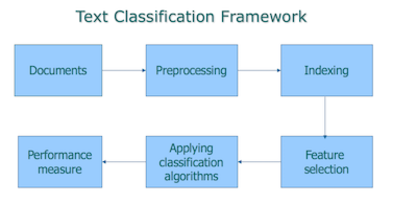
\includegraphics {finalgraph8.pdf}
  
\textbf{Naive Bayes Classification Technique:} Naive Bayes classifier, looks for differences of this sort by searching through text for words that are either (a) noticeably more likely to occur in A class, or (b) noticeably more likely to occur in B class. When a word is noticeably more likely to occur in one context rather than the other, its occurrence can be diagnostic of whether a new message is in A or B. If we see a single word that's more likely to occur in A than B, that's evidence that the token as a whole is in class A. 

Quite evidently, this approach is quite east of implement. Decent results are returned from this technique.

\textbf{Support Vector Machine:} The goal of Support vector machine (SVM for short) is to produce a model (based on the training data) which predicts the target values of the test data given only the test data attributes. SVM finds a linear separating hyperplane with the maximal margin. The instances that are closest to the maximum hyperplane are called support vectors. 

The kernel trick that could be used to solve problems with nonlinear decision boundaries. SVM allows you to use multiple different kernels to find nonlinear decision boundaries. 

\textbf{Decision Trees:} The root node in decision tree contains all the documents. Each internal node is a subset of documents separated by one attribute. Each node is further labelled with a predicate which can be applied at the parent. Finally, each leaf node is labelled with a class.Through the decision tree we were able get an accuracy of 

The confidence is used to compute the pessimistic upper bound of the error rate and is higher for pruning. J48 does not accept values greater then 0.5. 

\textbf{} 

\textbf{Perceptron(a review):} 
We use sklearn and numpy to develop a perceptron model as it is a binary classifier. We do this on just our tokens and try to understand the relation between testing and training errors. Further we adjust parameters such as the learning rate (eta). We observe that lower the learning rate higher the training accuracy. We receive an accuracy of 88.97\% on our training set. The average test error computes to 0.16\% and train error is 0.12\%. This process is performed on the basis of heldout validation. Perceptron is introduced as an alternative to existing approaches and can be explored further in future studies. 


   
\begin{table}[t]
\centering

 \begin{tabular}{c c c c} 
 \hline
 Character & Word position-Word \\ [0.5ex] 
 \hline\hline
 0.01235 & 50-me\\ 

 0.01079 & 48-makes\\

 0.00924  & 29-feel\\
 
 0.00883 & 40-i \\ 

 0.00836 & 46-lozenge \\

 0.00688 & 76-sick\\

 0.00655 & 67-prozac \\
 
 0.00638 & 42-it\\ 

 0.00621 & 49-making\\

 0.00619 & 63-pain\\

 0.00598 & 61-olanzapine\\
 
 0.00591 & 32-gain\\

 0.00587 & 93-zombie\\
 
 0.00543 & 89-weight \\ 

 0.00510 & 65-person\\

 \hline
\end{tabular}

\mycaption{Select Attributes 
\label{tbl-normalize}}
\aftertabspace
\end{table}





\subsection{Comparison and Review}
\label{sec-somethingnew}

\begin{table*}[t]
\centering
\begin{center}
 \begin{tabular}{c c c c c} 
 \toprule
 Type
 	& Correctly classified instances
		& Precisson
			& Recall
				& F-Measure
\\ 
 \midrule
Zero-R
 	& 89.4052\%
		& 0.799
			& 0.894
				& 0.844
 \\
 Naive Bayes
 	& 82.1561\%
		& 0.866
			& 0.822
			& 0.840
			 \\ 

 Decision Tree(J48) 
 	& 89.3123\% & 0.860 & 0.893 & 0.864\\
	
 Random Forest
 	& 89.4052\% & 0.860 & 0.894 & 0.861\\	
%% Requirements
%% 	& 	&  & Dependent \\ 
 
 Support Vector Machines
 	& 89.5911\%
		& 0.866
			& 0.896
			& 0.865
\\

 \bottomrule
\end{tabular}
\end{center}
\mycaption{Performance comparison of classification strategies without new tokens
\label{tbl-normalize}}
\aftertabspace
\end{table*}

\begin{table*}[t]
\centering
\begin{center}
 \begin{tabular}{c c c c c} 
 \toprule
 Type
 	& Correctly classified instances
		& Precisson
			& Recall
				& F-Measure
\\ 
 \midrule
Zero-R
 	&  89.4052\%
		& 0.799
			& 0.894
				& 0.844
 \\
 Naive Bayes
 	&  82.1561\%
		& 0.866
			& 0.822
			& 0.840
			 \\ 

 Decision Tree(J48) 
 	& 89.5911\% & 0.866 & 0.896 & 0.867\\
	
 Random Forest
 	& 89.5911\% & 0.865 & 0.896 & 0.858\\	
%% Requirements
%% 	& 	&  & Dependent \\ 
 
 Support Vector Machines
 	& 90.0558\%
		& 0.878
			& 0.901
			& 0.871
\\

 \bottomrule
\end{tabular}
\end{center}
\mycaption{Performance comparison of classification with new tokens
\label{tbl-normalize}}
\aftertabspace
\end{table*}
  


An overview of the attributes is shown in \textbf {Table 3} and \textbf{Table 4}.
Accuracy is computed as in equation  \eqref{eq:accuracy}.

\begin{equation}
\label{eq:accuracy}
Accuracy = \frac{\mathit{Total\ correct\ predictions}}{\mathit{Number\ of\ test\ predictions}}
\end{equation}


Precision is computed as in equation \eqref{eq:precision}.

\begin{equation}
\label{eq:precision}
Precision = \frac{\mathit{Number\ of\ correct\ predictions}}{\mathit{Total\ number\ of\ predictions}}
\end{equation}

Recall is computed as in equation \eqref{eq:recall}.

\begin{equation}
\label{eq:recall}
Recall = \frac{\mathit{Number\ of\ correct\ words}}{\mathit{Total\ number\ of\ words}}
\end{equation}

F-measure is computed as in equation  \eqref{eq:fmeasure}.

\begin{equation}
\label{eq:fmeasure}
F-Measure = \frac{\mathit{2\ *\ Precision\ *\ Recall}}{\mathit{Precison\ +\ Recall}}
\end{equation}

\myparagraph{Naive Bayes} The low accuracy rate can be attributed to the assumption of class conditional independence. As we know that in practical systems, there is a dependency between variables. We were unable to find a way of modelling these dependencies directly. Upon further research it appeared that Bayesian Belief Networks were to be considered for handling there dependencies. Thus, the assumptions outweigh the ease of implementation when it comes to critical comparison with other techniques.
On observing the true positive rate i.e., 0.482 we realise that this is quite high. Further the number of Y classes(52) i.e. predicted Y are very close to the N(59) predicted (Data from the confusion matrix). The higher number of Y terms explain the positive relation with a lower value in correctly classified instances. The false positive rate for N class is 0.518, thus reducing the number of correctly classified instances. 

\myparagraph{Support Vector} We found SVMs as much slower compared to other techniques. The computational cost of SVM was rather high. This can be explained as large quadratic optimisation have to be solved on a large set of variables. This could be explained by the fact that SVMs training is associated with Lagrangian dual instead of primal problem. In our observation, SVM produce very accurate classifiers, the highest among all the techniques discussed. It would be important to note that SVMs generally are less overfitting and robust to noise.

SVM map to a high dimensional space, thus having a strong bias in that space. Thus, there is a rich proportion of optimisation in SVM. Under WEKA we found that when 10-fold cross validation is performed on the Normalized Poly Kernel, we obtain 1161 support vectors of which 86.4\% are cached. 

\myparagraph{Decision Trees} 
The default confidence value in J48 is 0.25. It seems that there is an inverse relationship between the confidence pruning and tree pruning. Higher the value of confidence pruning, less the tree is pruned. 
Decision tree tries to make the optimal tree at every step. An observation between the time to train versus the time to test is made. The time for training is substantially higher, perhaps sometimes the highest across all the techniques. However, the testing is almost instantaneous once the model is trained. 

The confusion matrix of decision tree reveals the bias in information gain which favours attributes with more level. In the confusion matrix we see large amounts of N predicted where the classifier has a True Positive of 0.986.

We make the observation on the percentage split of decision tree. By default, WEKA maintain this number as 66\% and we are able to make 1076 observations. This gives us an accuracy of 88.29\%. However, say we increase the percentage split to 90\%, then the number of instances are decreased to 317 with an accuracy of 90.85\%. This shows us the impact of pruning of the trees and helps us validate our understanding of generating better results with smaller trees. 






















  


\section{{\itshape Mining Twitter for Adverse Drug Reaction Mentions:} A Corpus and Classification Benchmark(Research Review)}

In this section, we review and try to understand the work of {\citet{gmctw14}} on the same problem. The corpus was manually annotated and created through extraction of tweets related to 74 drugs, using their brand and generic names, and phonetic misspellings. These were annotated for the presence of ADRs (a binary attribute for each tweet), the location/span of the reaction mentions, and the UMLS concept IDs for the ADR mentions. Further, they extended the drug list to include misspelled drug names. This was critical to obtaining relevant tweets, as drug names are often misspelled in social media. They generated the misspellings through a phonetic spelling filter.

Additionally, the corpus was not only set for the presence or absence of ADR mentions, but also to identify the span of the expressions conveying individual ADRs, and to map them to formal medical terminology. Two annotators were manually annotated the processed tweets: binary annotation of ADRs and full ADR annotations. The result would be for, 'weight gain', 'gained 20 pounds', 'put on too much weight', or 'fat fat fat' would all be annotated to a general concept ID for 'weight gain'. 

For the ADR detection, they used NB and SVM classifiers for the binary classification task. In SVM only the was used linear kernel with no attempts at parameter optimisation. Three sub datasets were created changing the proportions of HasADR and NoADR. In dataset1 both the parameters were equal, in the second HasADR was greater than NoADR and in the third NoADR was greater. 

Mapping an annotated concept to semantically equivalent UMLS concept IDs for an agreement was needed. Inter-annotator agreement (IAA) using Cohen's kappa was computed for binary annotations. The largest source of error came from the differences in concept IDs chosen. Some term used by the user, such as 'hangover' may or may not be an ADR. Also the span has to be considered.

Performance of accuracy in SVM and NB are compared. Majority labelling is performed in which every test instance to the majority class in the test set. Both classifiers perform better than the majority labelling baseline. An observation that the classifier accuracies increase slightly as the proportion of the majority class increases is made. The study is concluded as a stepping stone into classification performance while maintaining the goal of deep semantic learning on tweets. 




%\section{Experiments}
\label{sec-experiments}

\todo{Where much of the hard work is}

Down, down, down.
There was nothing else to do, so Alice soon began talking again.
'Dinah'll miss me very much to-night, I should think!'
(Dinah was the cat.)
'I hope they'll remember her saucer of milk at tea-time.
Dinah my dear!
I wish you were down here with me!
There are no mice in the air, I'm afraid, but you might catch a bat,
and that's very like a mouse, you know.
But do cats eat bats, I wonder?'
And here Alice began to get rather sleepy, and went on saying to
herself, in a dreamy sort of way, 'Do cats eat bats?
Do cats eat bats?'
and sometimes, 'Do bats eat cats?'
for, you see, as she couldn't answer either question, it didn't much
matter which way she put it.
She felt that she was dozing off, and had just begun to dream that
she was walking hand in hand with Dinah, and saying to her very
earnestly, 'Now, Dinah, tell me the truth: did you ever eat a bat?'
when suddenly, thump!
thump!
down she came upon a heap of sticks and dry leaves, and the fall was
over.

Alice was not a bit hurt, and she jumped up on to her feet in a
moment: she looked up, but it was all dark overhead; before her was
another long passage, and the White Rabbit was still in sight,
hurrying down it.
There was not a moment to be lost: away went Alice like the wind, and
was just in time to hear it say, as it turned a corner, 'Oh my ears
and whiskers, how late it's getting!'
She was close behind it when she turned the corner, but the Rabbit
was no longer to be seen: she found herself in a long, low hall,
which was lit up by a row of lamps hanging from the roof.

There were doors all round the hall, but they were all locked; and
when Alice had been all the way down one side and up the other,
trying every door, she walked sadly down the middle, wondering how
she was ever to get out again.


%\section{Conclusions}
\label{sec-conclusions}

Suddenly she came upon a little three-legged table, all made of solid
glass; there was nothing on it except a tiny golden key, and Alice's
first thought was that it might belong to one of the doors of the
hall; but, alas!
either the locks were too large, or the key was too small, but at any
rate it would not open any of them.
However, on the second time round, she came upon a low curtain she
had not noticed before, and behind it was a little door about fifteen
inches high: she tried the little golden key in the lock, and to her
great delight it fitted!

Alice opened the door and found that it led into a small passage, not
much larger than a rat-hole: she knelt down and looked along the
passage into the loveliest garden you ever saw.
How she longed to get out of that dark hall, and wander about among
those beds of bright flowers and those cool fountains, but she could
not even get her head through the doorway; 'and even if my head would
go through,' thought poor Alice, 'it would be of very little use
without my shoulders.
Oh, how I wish I could shut up like a telescope!
I think I could, if I only knew how to begin.'
For, you see, so many out-of-the-way things had happened lately, that
Alice had begun to think that very few things indeed were really
impossible.

There seemed to be no use in waiting by the little door, so she went
back to the table, half hoping she might find another key on it, or
at any rate a book of rules for shutting people up like telescopes:
this time she found a little bottle on it, ('which certainly was not
here before,' said Alice,) and round the neck of the bottle was a
paper label, with the words 'DRINK ME' beautifully printed on it in
large letters.

It was all very well to say 'Drink me,' but the wise little Alice was
not going to do THAT in a hurry. 'No, I'll look first,' she said, 'and
see whether it's marked "poison" or not'; for she had read several nice
little histories about children who had got burnt, and eaten up by wild
beasts and other unpleasant things, all because they WOULD not remember
the simple rules their friends had taught them: such as, that a red-hot
poker will burn you if you hold it too long; and that if you cut your
finger VERY deeply with a knife, it usually bleeds; and she had never
forgotten that, if you drink much from a bottle marked 'poison,' it is
almost certain to disagree with you, sooner or later.

However, this bottle was NOT marked 'poison,' so Alice ventured to
taste it, and finding it very nice, (it had, in fact, a sort of mixed
flavour of cherry-tart, custard, pine-apple, roast turkey, toffee,
and hot buttered toast,) she very soon finished it off.


%-------------------------------------------------------------------%



\balance %% <- doesn't work with footnotes
%% \bibliographystyle{ACM-Reference-Format}
\bibliographystyle{abbrvnat}
\bibliography{strings-shrt,local} 

\end{document}
